\section{CLIP with Prompt Engineering}
\begin{figure}[ht]
    \centering
    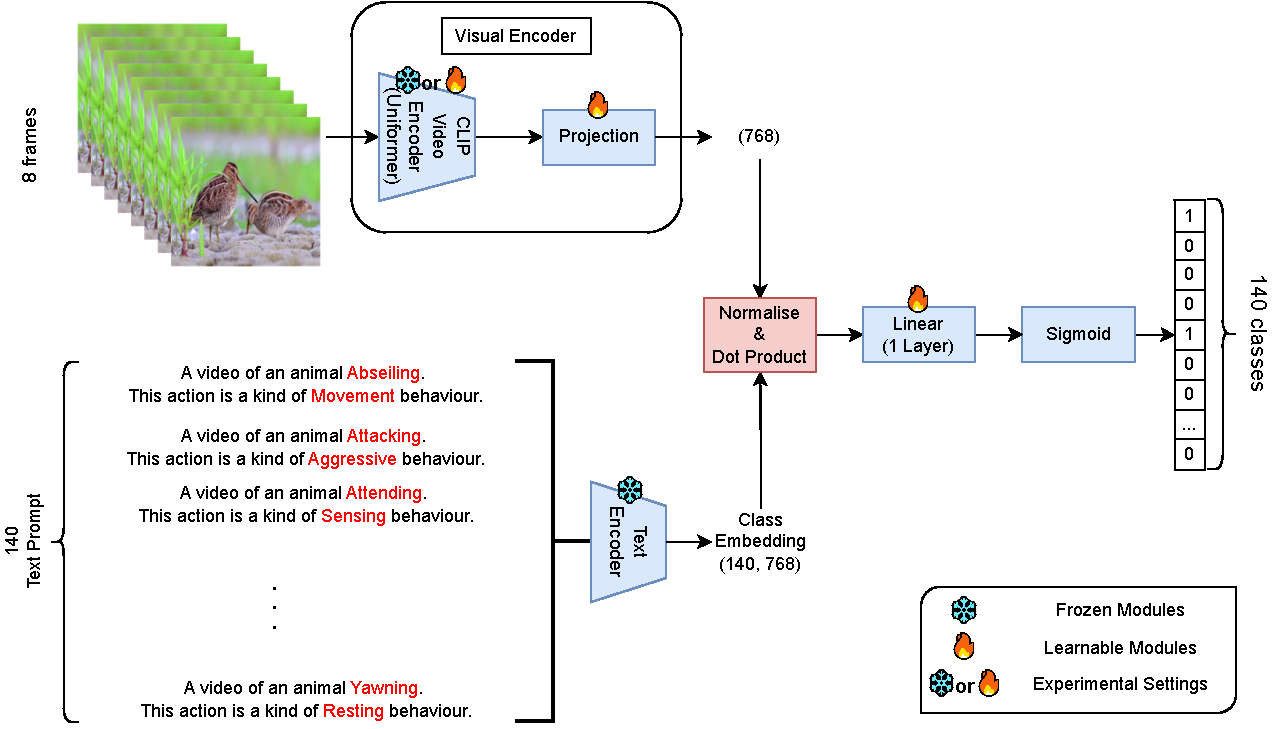
\includegraphics[width=1.0\textwidth]{assets/imgs/3_1_ModelStructureVC}
    \caption[CLIP Action Recognition Model Stucture 1]{This Chart illustrates the model stucture of applying Video CLIP and prompt engineering for action recognition.}
    \label{fig:modelstructic1}
\end{figure}

\begin{figure}[ht]
    \centering
    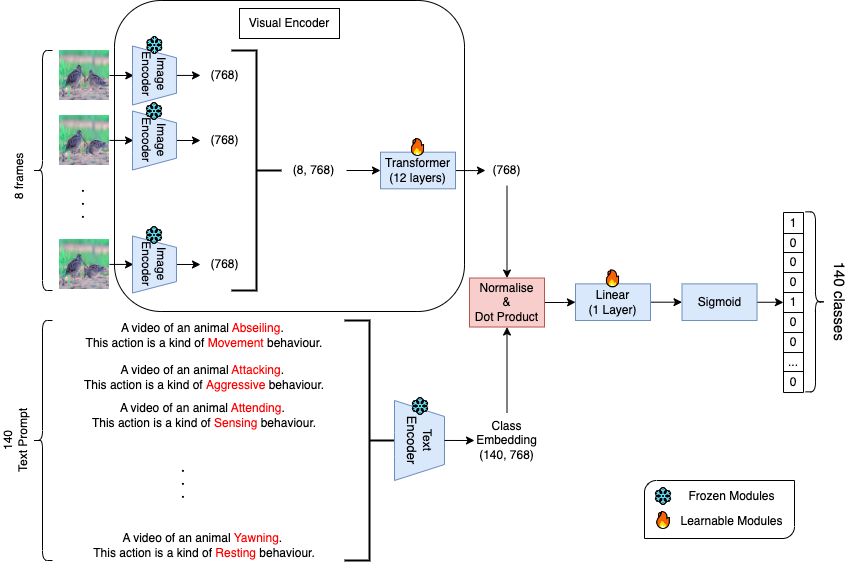
\includegraphics[width=1.0\textwidth]{assets/imgs/3_2_ModelStructureIC}
    \caption[CLIP Action Recognition Model Stucture 2]{This Chart illustrates the model stucture of applying Image CLIP and prompt engineering for action recognition.}
    \label{fig:modelstructic2}
\end{figure}

I designed two model structures for action recognition to test the performance of Image CLIP \parencite{radford2021learning} and and Video CLIP \parencite{wang2022internvideo}. Figure \ref{fig:modelstructic1} and \ref{fig:modelstructic2} illustrates the two model structures, which uses CLIP and prompt engineering for action recognition. The models both take video and text prompt as input. The prompt template and its enbedding distribution is shown in Figure \ref{fig:1_1_ClassEmbeddingInternVideo}. 

Before training begins, in order to accelerate the process, the class embeddings of size $(140, 768)$ are pre-calculated by text encoder pretrained by InternVideo based on the prompt template, action name, and category. This is done since the text encoder is frozen, and the weights are not updated. 

Figure \ref{fig:modelstructic1} use video encoder of InternVideo clip module, which is Uniformer, as its visual encoder. In order to evaluate the structure fairly, I experiment the two model settings on this structure: Video Clip train on all vision layers, and Video Clip train only on projection layers. Figure \ref{fig:modelstructic2} uses image encoder of CLIP as its visual encoder. In order to encode the 8 frames into a video embeddings, 8 image embeddings encoded by image CLIP should be further passed through 12 layers post-transformer with a pooling layer to produce a 768-dimensional video embedding.

In contrast to multiclass classification, this is multilabel classification, meaning that a video may belong to more than one class. Therefore, I add a linear layer as a buffer to help the model fit better. Finally, the output logits of the linear layer are then pass through a sigmoid function to determine the probability of each class. 

\section{AFRICAN}
The whole AFRICAN consist of two stage: pretraining and action recognition. The pretraining stage is to train the model to distinguish whether two images are augmented from the same frame in a video or not. The action recognition stage is utilise the pretrained model to extract more meaningful embedding for action recognition. 

\subsection{AFRICAN Pretraining}

\begin{figure}[ht]
    \centering
    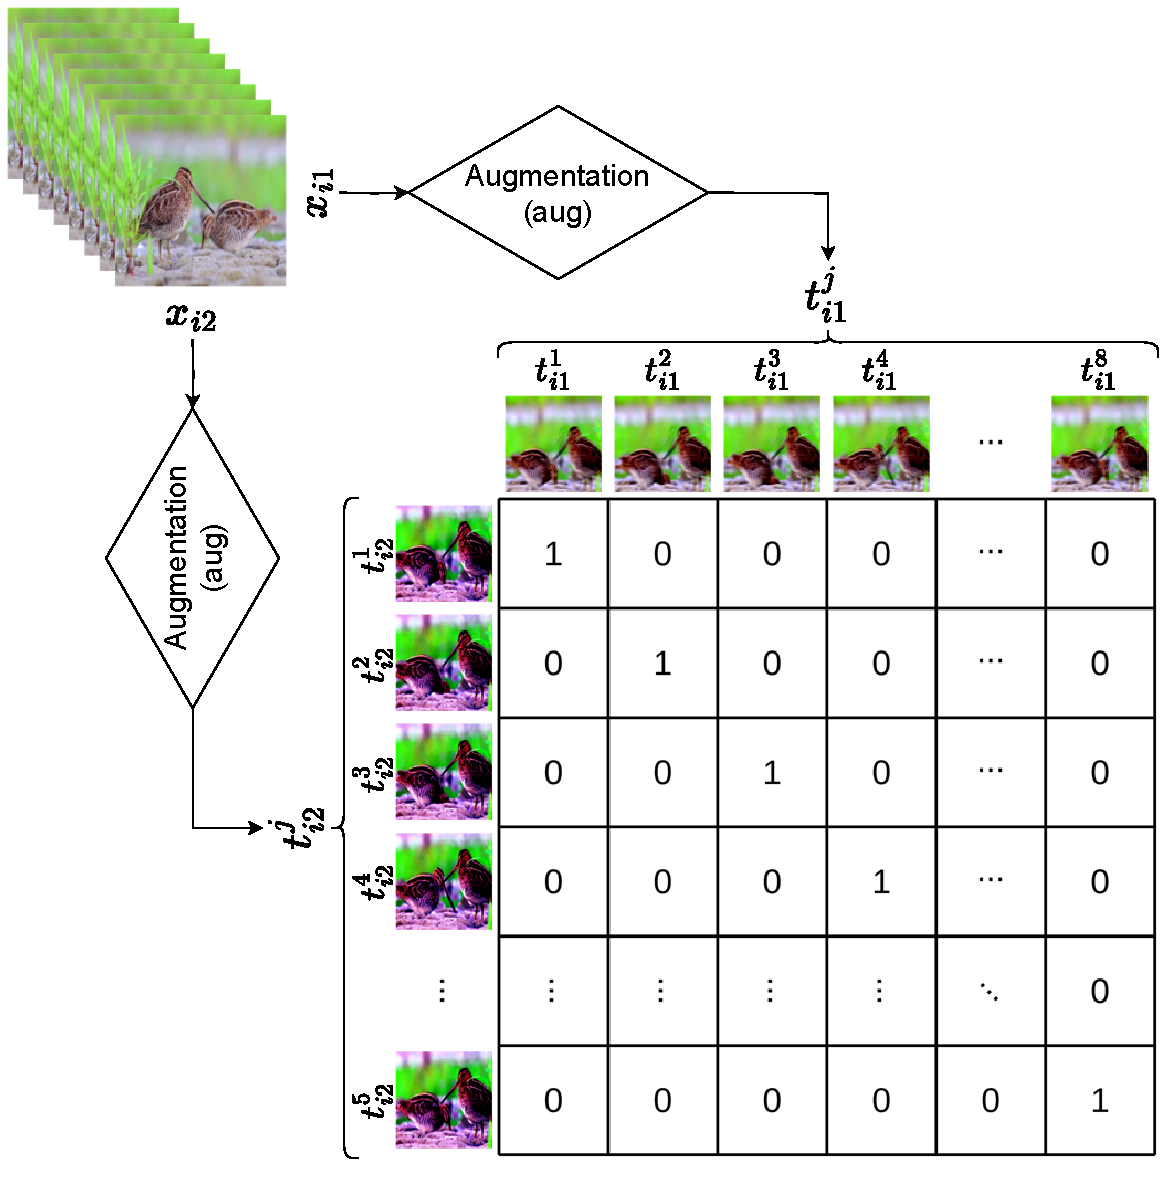
\includegraphics[width=0.6\textwidth]{assets/imgs/3_3_ConstrastiveSimilarityMatrix}
    \caption[Operation of AFRICAN pretraining]{This chart illustrates the operation of AFRICAN pretraining.}
f\label{fig:modelstructafsim}
\end{figure}

At the pretraining stage, AFRICAN apply a contrastive learning techniques to distinguish whether two images are augmented from the samefframe in a video or not. Figure \ref{fig:modelstructafsim} illustrates the batch operation of the model. The input for forwarding is a video sample $x_i$, where $i$ denotes the $i$-th sample in the dataset. $x_i$ is then copied twice into $x_{i1}$ and $x_{i2}$, which then independently pass through the same video augmentation function $aug(\cdot)$ with different random seeds, as shown in Equations \ref{eq:aug1} and \ref{eq:aug2}. 

\begin{equation}
    \label{eq:aug1}
    t_{i1} = aug(x_{i1})
\end{equation}
\begin{equation}
    \label{eq:aug2}
    t_{i2} = aug(x_{i2})
\end{equation}

After the transformation, $t_{i1}$ and $t_{i2}$ are separated into $j$ frames, denoted as $t_{i1}^j$ and $t_{i2}^j$. In this research, 8 frames are sampled in from a video in a vatch. Each frame will go through the same image encoder $f(\cdot)$ to be encoded into embeddings $e_{i1}^j$ and $e_{i2}^j$, as shown in Equations \ref{eq:enc1} and \ref{eq:enc2}.

\begin{equation}
    \label{eq:enc1}
    e_{i1}^j = f(t_{i1}^j)
\end{equation}
\begin{equation}
    \label{eq:enc2}
    e_{i2}^j = f(t_{i2}^j)
\end{equation}

Afterwards, the similarity between the image embeddings is calculated by normalisation and dot product, as shown in Equation \ref{eq:sim}, where $k$ denotes the frame index of $e_{i1}$ and $l$ denotes the frame index of $e_{i2}$. The numbers in the matrix in Figure \ref{fig:modelstructafsim} represent the learning targets for different image pair inputs. The diagonal line represents the frame pairs augmented from the same frames, while other numbers indicate pairs of images from different source frames. 

\begin{equation}
    \label{eq:sim}
    t_{i}^{kl} = norm(e_{i1}^{k}) \cdot norm(e_{i2}^{l})
\end{equation}




\subsection{AFRICAN for Action Recognition}

\begin{figure}[ht]
    \centering
    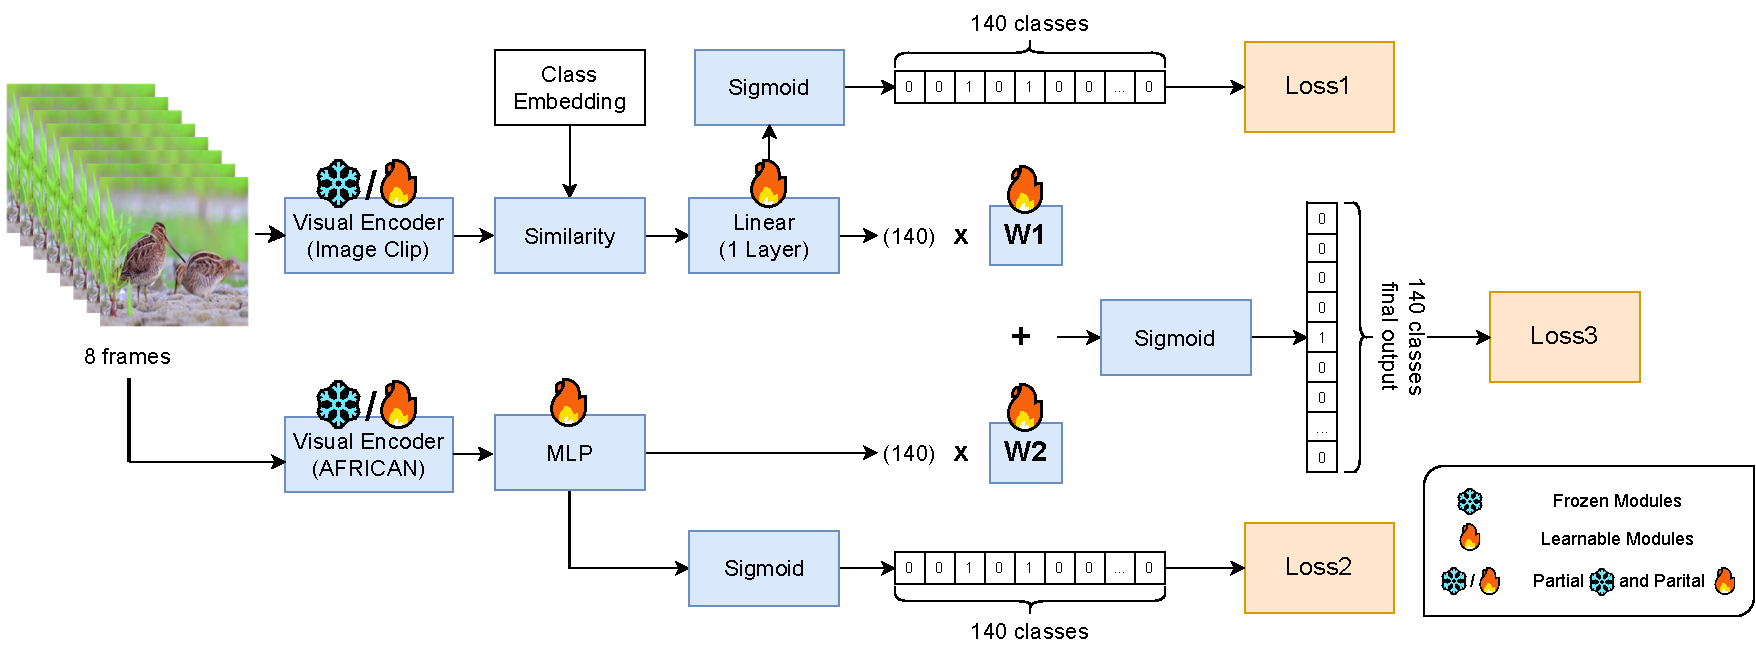
\includegraphics[width=1.0\textwidth]{assets/imgs/3_4_ModelStructureAF}
    \caption[Operation of AFRICAN for action recognition]{This chart illustrates the operation of AFRICAN for action recognition.}
    \label{fig:modelstructaf_ar}
\end{figure}

% TODO: further discussion is in the ablation study
Figure \ref{fig:modelstructaf_ar} illustrates the operation of AFRICAN for action recognition. The whole structrue consist of two streams. The upper stream is the pretrained CLIP stream, the lower stream is the pretrained AFRICAN stream.
In the pretrained CLIP stream, the visual encoder and class embedding is the same as the visual encoder and class embedding in Figure \ref{fig:modelstructic2}. Because the structure of image CLIP is able to achieve better performance than video CLIP, I use the image CLIP here as the visual encoder in the clip stream. 

In the pretrained AFRICAN stream, the structure of visual encoder is the same as the pretrained CLIP stream but with pretrained AFRICAN weights. Since the AFRICAN is not pretrained by the visual-text multimodality model like CLIP, there is no corresponding class embedding. Therefore, a commonly used structure, multilayer perceptron (MLP), is used to do map the embedding and one-hot encoding. The 3-layer MLP takes the video embedding as input and output a 140 dimensional logits, which then pass through sigmoid function to do the classification.

After the logits, the input of the sigmoid function, are obtained in the two streams, they are separatedly used for prediction, which are used to compute the loss1 and loss2. At the same time, the logits of both streams will be multiplied by a 140 dimensional weights to determine the importance of each class for both streams, which is followed by an addition to produce the final prediction, which is used to compute the loss3. Finally, the loss1, loss2, and loss3 are added together to do the backpropagation. 





